\section{What is HIVE}

HIVE try to solve traditional problems of vocabularies in digital environments. We can enumerate these problems as follow:

\begin{itemize}
\item Concept Retrieval
\item Automatic annotation
\item RIA technology for vocabulary server Web User Interface
\item Linked Data for Concepts based on SPARQL end points
\end{itemize}

In the next sections we will explain how HIVE solves these problems, to offer a 
methodology and tool which allows vocabularies use on the Web.

HIVE Core is a SKOS Core based library written entirely in Java. It is a technology suitable for nearly any application that requires 
vocabularies management.

\section{HIVE core architecture}

HIVE Core allow users to access to the vocabularies in different ways, As you can see in the image below, the system can be queried in two different ways:

Natural Language Interface
SPARQL interface

HIVE integrate different libraries to allow these access. Natural Language interface allow us to use keyword based queries to retrieve concepts from the vocabularies. 
This interface is based on Lucene, so each query is fired against a Lucene index where the concepts are stored.

\begin{figure}
\centering
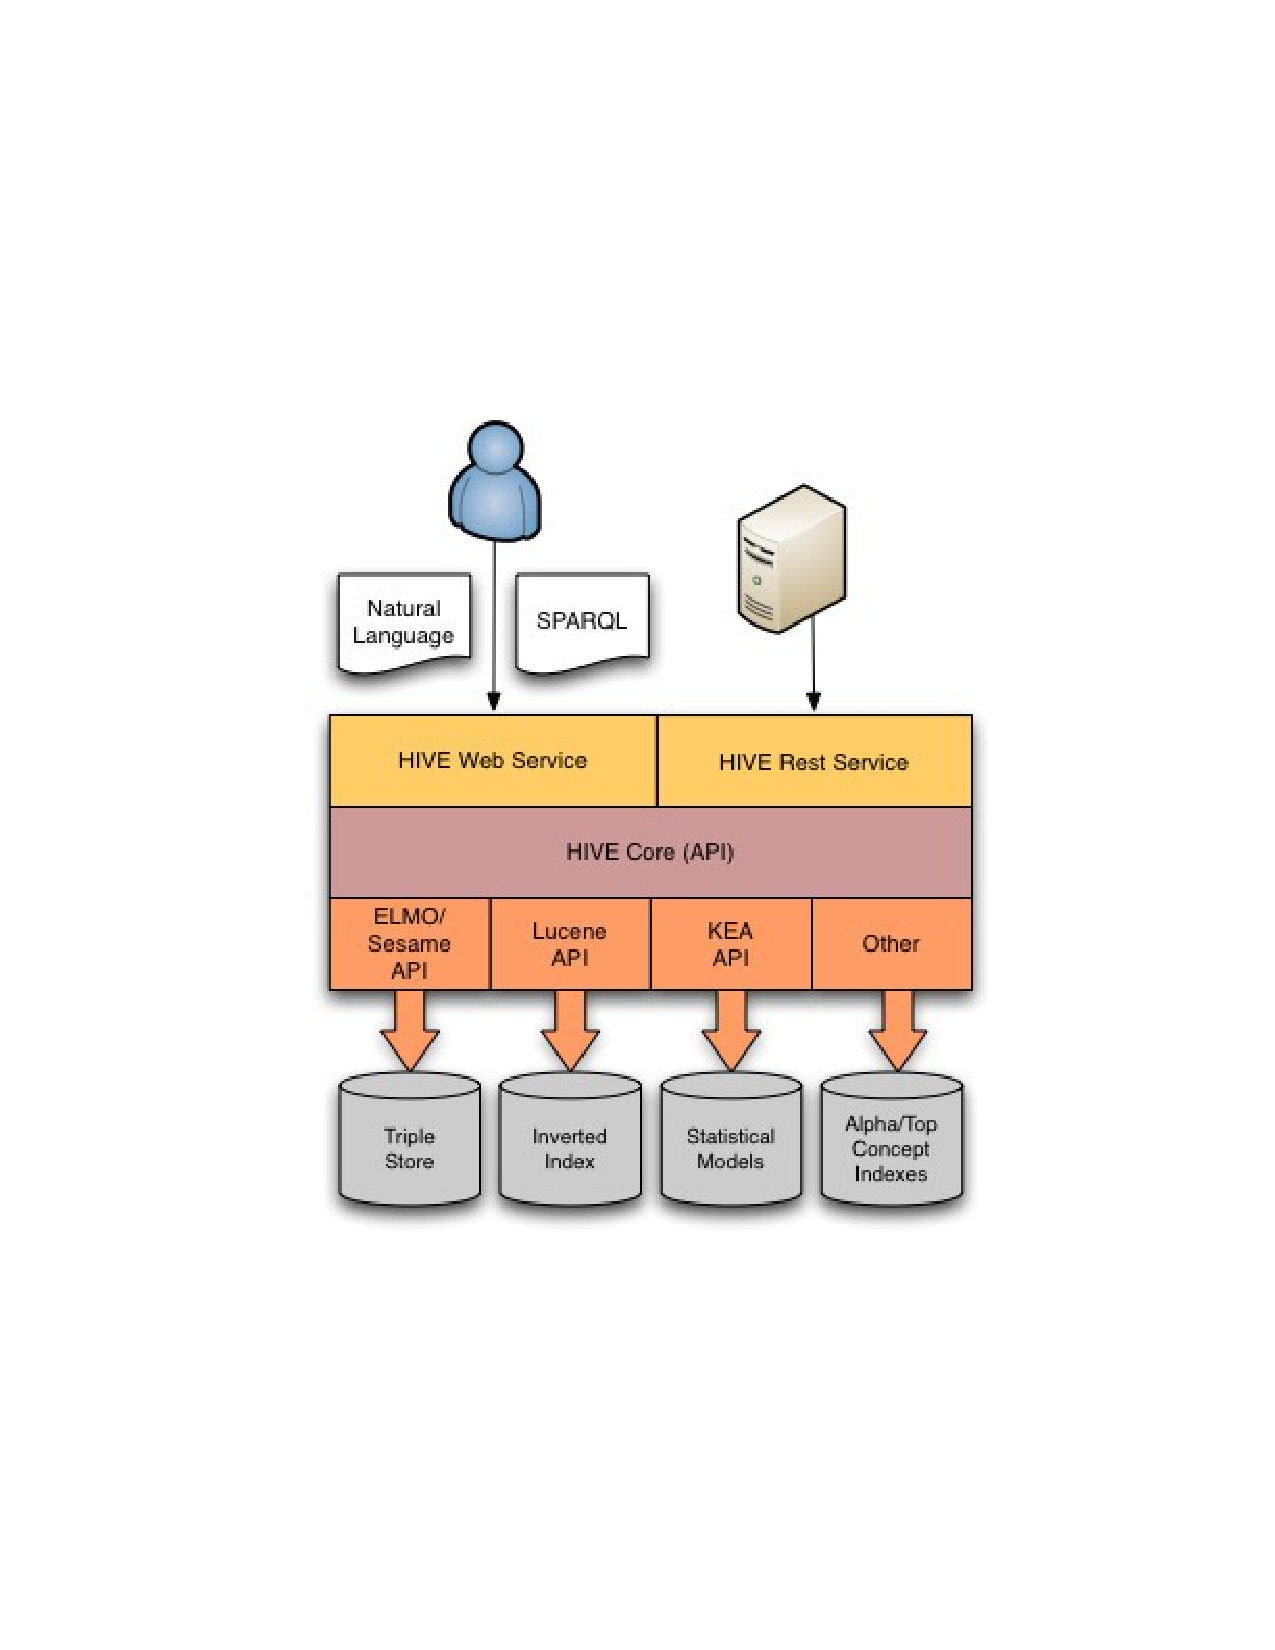
\includegraphics[width=400pt]{img/hive-architecture.pdf}
\caption{HIVE Core architecture}
\label{hivearchitecture}
\end{figure}
 
\section{Loading vocabularies from SKOS Core}\label{configuration}

Loading new vocabularies in HIVE is quite simple. HIVE is able to load any vocabulary in SKOS Core format from RDF files. So If we have 
a vocabulary in a file with SKOS Core format, you could import it into HIVE very easily.

To import a vocabulary you only need execute AdminVocabularies class, which have a main method that implement the basic importation. 
The parameters to execute this class are two:

1- the path to the ../conf directory for HIVE, where the configuration file for the HIVE server and for every vocabulary are. 
In each vocabulary configuration file you have to define where do you want store the different databases that HIVE will use to store the 
vocabulary and you can also define the location of the RDF file from where you want import the vocabulary.

The format of the file for the example of lcsh.properties file would be the following:

\begin{verbatim}
 #Vocabularies data
name = LCSH
longName = Library of Congress Subject Headings
uri = http://id.loc.gov/authorities

#Sesame Store
store = /home/hive/hive-data/lcsh/lcshStore

#Lucene Inverted Index
index = /home/hive/hive-data/lcsh/lcshIndex

#Alphabetical Index
alpha_file = /home/hive/hive-data/lcsh/lcshAlphaIndex

#Top Concept Index
top_concept_file = /home/hive/hive-data/lcsh/lcshTopConceptIndex

#Dummy tagger data files
lingpipe_model = /home/hive/hive-data/lingpipe/postagger/models/medtagModel

#KEA data files
stopwords = /home/hive/hive-data/lcsh/lcshKEA/data/stopwords/stopwords_en.txt
kea_training_set = /home/hive/hive-data/lcsh/lcshKEA/train
kea_test_set = /home/hive/hive-data/lcsh/lcshKEA/test
rdf_file = /home/hive/hive-data/lcsh/lcsh.rdf
kea_model = /home/hive/hive-data/lcsh/lcshKEA/lcsh
\end{verbatim}

You should have one file like this for every vocabulary that you want load in HIVE.

\begin{verbatim}
 		String configpath = args[0];
		String vocabularyName = args[1].toLowerCase();

		SKOSScheme schema = new SKOSSchemeImpl(configpath, vocabularyName, true);

		ImporterFactory.selectImporter(ImporterFactory.SKOSIMPORTER);
		Importer importer = ImporterFactory.getImporter(schema);
		importer.importThesaurustoDB();
		importer.importThesaurustoInvertedIndex();
		importer.close();
		System.out.println("Import finished");
//		if (args[2].equals("train")) {
//			TaggerTrainer trainer = new TaggerTrainer(schema);
//			trainer.trainAutomaticIndexingModule();
// 		}
	}
\end{verbatim}

\subsection{Creating databases and indices}

The AdminVocabularies class use an SKOSScheme that represent a SKOS vocabulary into HIVE and a Importer which implement all the importation 
process. Importer are implemented as a Factory, although at this moment there is only implemented one importer for SKOS format. 
Once we have decide what importer we want to use we can call different methods. Every method is related with a different kind of storage:

importThesaurustoDB(): this method implement the interface to add data to the Sesame database. HIVE use NativeStore, so every vocabulary imported using this 
method will be stored on your file system with this format.
importThesaurustoInvertedIndex(): this method create a Lucene index to store the information about concepts. At this point we are following a document 
oriented approach to represent concepts in the inverted index, so each concept is actually represented as a document with different fields. Each field 
represent the different elements which we can find in a vocabulary, preferred term, broader terms, scope notes, etc.

HIVE importer create to additional indexes for every vocabulary, in order to optimize the access to different representations of the same vocabulary. These 
two additional indexes are the following:

Alphabetical index: This index is an alphabetically ordered list which make easier represent concepts in a alphabetical way
Hierarchical index: This index allow us to create hierarchical representation of the data in order to implement representations based on the hierarchical 
structure of the vocabularies.

Both indexes are created after the inverted index. 

All theses indexes and databases can be stored wherever you need in your file systems. The location of each database and index have to be defines in the properties 
file what we have for every vocabulary in the ../conf directory.

\subsection{Creating training data for automatic metadata generation}

HIVE automatic metadata generation system is based in KEA. When a vocabulary is imported we have the chance to create a model to use the vocabulary for automatic 
metadata generation. In this section we will explain how create this model and when locate the information about this model. The theoretical framework of KEA and 
how the model is used for automatic metadata generation will be explained in chapter \ref{kea}.

KEA algorithm is based on machine learning techniques and more specifically in a Naïve Bayes based classification system. Machine Learning algorithms use to need 
two different sets of data: Training data and Test data.

Training data are used to build an statistical model which is used by the algorithm to recognize positive and negative examples. This statistical models use to 
be based on real world example, so for automatic metadata generation we will use a corpus of documents where keywords and metadata has been assigned by hand.

\section{SKOS Server}


SKOSServer is the high level classes that we have to instantiate to get up the Vocabulary server:

\begin{verbatim}
 SKOSServer server = 
  new SKOSServerImpl("/home/hive/workspace/hive-core/conf/vocabularies");
\end{verbatim}
 
where the method's argument makes reference to the configuration file where the names of the thesauri to load is written.

\begin{figure}
\centering
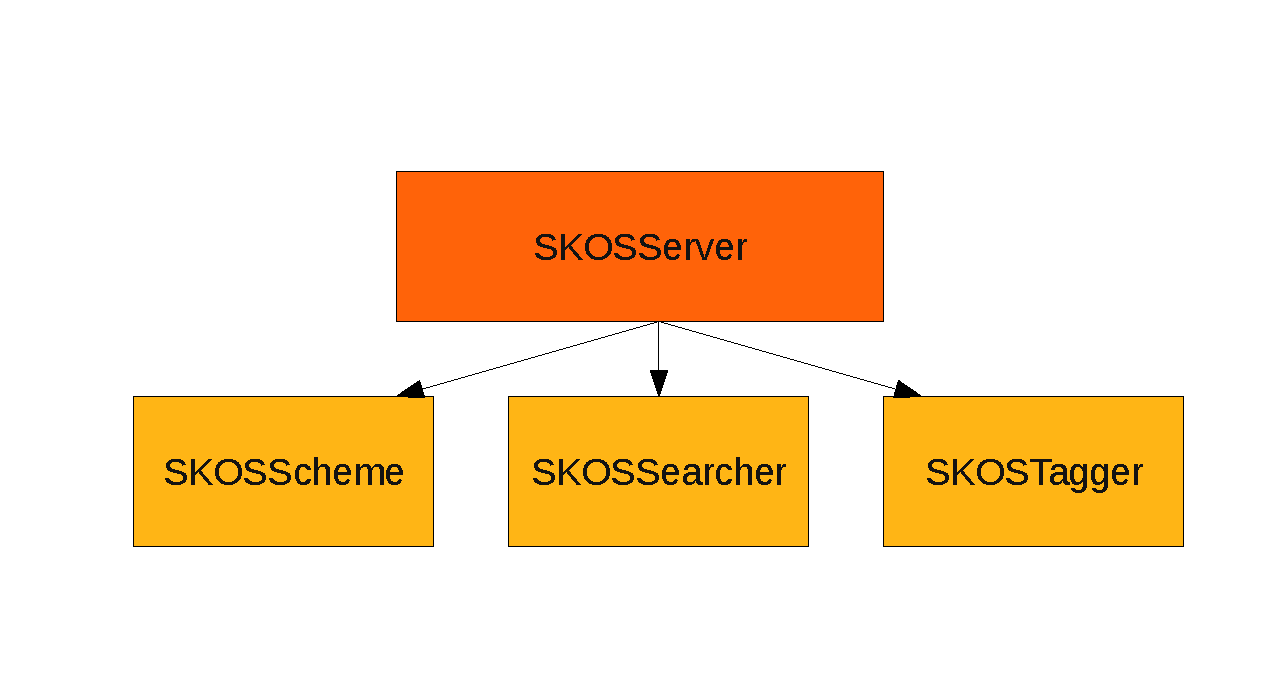
\includegraphics[width=400pt]{img/skosserver.pdf}
\caption{SKOS Server}
\label{skosserver}
\end{figure}

SKOSServer manages the three basic classes which take the work to implement the HIVE basic functionalities: Concept Search 
(SKOSSearcher), Vocabularies management (SKOSScheme) and indexing SKOSTagger.

Any of theses classes are actually interfaces which are implemented using different libraries,

\section{SKOS Scheme}

Every vocabulary in modeled in HIVE using SKOSScheme class. This class contains information about the vocabularies 
and some methods to manage them.

We can get information about statistics for every vocabulary, number of terms, and relations, updates, etc. The following piece of code show you how to do that:

\begin{verbatim}
TreeMap<String, SKOSScheme> vocabularies = server.getSKOSSchemas();
Set<String> keys = vocabularies.keySet();
Iterator<String> it = keys.iterator();
	  while (it.hasNext()) {
		  SKOSScheme voc = vocabularies.get(it.next());
		  System.out.println("NAME: " + voc.getName());
		  System.out.println("\t LONG NAME: " + voc.getLongName());
		  System.out.println("\t NUMBER OF CONCEPTS: "
		      + voc.getNumberOfConcepts());
		  System.out.println("\t NUMBER OF RELATIONS: "
		      + voc.getNumberOfRelations());
		  System.out.println("\t DATE: " + voc.getLastDate());
		  System.out.println();
		  System.out.println("\t SIZE: " + voc.getSubAlphaIndex("a").size());
		  System.out.println();
		  System.out.println("\t TOP CONCEPTS: "
		      + voc.getTopConceptIndex().size());
	  }
\end{verbatim}


\section{Search functionalities with SKOSSearcher}

SKOSSearcher, is the interface which defines the search functionalities in HIVE. Theses functionalities can be divided into two different 
kind of search:

\begin{itemize}
 \item Formal Search
 \item Keyword based search
\end{itemize}

\subsection{Formal Search based on SPARQL}

Formal search is based on SPARQL, a formal language to get information from RDF databases. SPARQL is the standard query language for 
Semantic Web application and it is useful to implemented Web Services based on SPARQL end points, and so allowing third part application 
retrieve information from a RDF database.

\begin{verbatim}
 searcher.SPARQLSelect(
  "SELECT ?s ?p ?p WHERE {?s ?p ?o} LIMIT 10", 
  "nbii");
\end{verbatim}

\begin{verbatim}
 searcher.SPARQLSelect(
  "PREFIX skos: <http://www.w3.org/2004/02/skos/core#> 
  SELECT ?s ?p ?o WHERE {  ?s ?p ?o . ?s skos:prefLabel \"Damage\" .}",
  "nbii");
\end{verbatim}

\begin{verbatim}
 searcher.SPARQLSelect(
  "PREFIX skos: <http://www.w3.org/2004/02/skos/core#> 
  SELECT ?uri ?label WHERE { <http://thesaurus.nbii.gov/nbii#Mud> 
  skos:broader ?uri . ?uri skos:prefLabel ?label}",
  "nbii");
\end{verbatim}

\subsection{Keyword based search}

Keyword based search is based in natural language search, so the user of the system can write queries without any constraint. HIVE keyword 
based search is based our research on Concept and Entity retrieval which has been described in José R. Pérez-Agüera, Javier Arroyo, 
Jane Greenberg, Joaquin Perez-Iglesias and Victor Fresno. Using BM25F for Semantic Search. Semantic Search Workshop at the 19th Int. 
World Wide Web Conference WWW2010 April 26, 2010 (Workshop Day), Raleigh, NC, USA

\begin{verbatim}
System.out.println("Search by keyword:");
List<SKOSConcept> ranking = searcher.searchConceptByKeyword("accidents");
System.out.println("Results in SKOSServer: " + ranking.size());
String uri = "";
String lp = "";
  for (SKOSConcept c : ranking) {
    uri = c.getQName().getNamespaceURI();
    lp = c.getQName().getLocalPart();
    QName qname = new QName(uri, lp);
    String origin = server.getOrigin(qname);
    if (origin.toLowerCase().equals("nbii")) {
      System.out.println("PrefLabel: " + c.getPrefLabel());
      System.out.println("\t URI: " + uri + " Local part: " + lp);
      System.out.println("\t Origin: " + server.getOrigin(qname));
    }
  }
\end{verbatim}

\subsection{URI based search}

\begin{verbatim}
System.out.println("Search by URI:");
SKOSConcept c2 = searcher.searchConceptByURI(
  "http://thesaurus.nbii.gov/nbii#", "Enzymatic-activity");
Concept c2 = searcher.searchConceptByURI(uri, lp);
List<String> alt = c2.getAltLabels();
System.out.println("PrefLabel: " + c2.getPrefLabel());
for (String a : alt) {
  System.out.println("\t altLabel: " + a);
}
System.out.println("\t Origin: " + server.getOrigin(c2));
System.out.println("\t SKOS Format: \n" + c2.getSKOSFormat());
\end{verbatim}

\begin{verbatim}
/**
/ * Get Children by URI test
 */
SKOSConcept con = searcher.searchConceptByURI(
    "http://id.loc.gov/authorities/sh2001009743#", "concept");
TreeMap<String,QName> children = searcher.searchChildrenByURI(
  "http://id.loc.gov/authorities/sh2001009743#", "concept");
for (String c : children.keySet()) {
  System.out.println("prefLabel: " + c);
}
\end{verbatim}


\section{Tagging documents with SKOS Tagger}

One of the most important features of HIVE is the module for automatic metadata extraction. Use this functionality is quite easy using the SKOSTagger class. 
This class is accesed via SKOSServer using the method getSKOSTagger().

Once we have an SKOSTagger we can use the method getTags(), to get the keywords for a given document. The arguments required for this method are the source 
of the text, usually a document, the list of vocabularies to normalize the keywords and a SKOSSearcher object. Following there is an example about how to use HIVE tagger.

\begin{verbatim}
SKOSTagger tagger = server.getSKOSTagger();

String source = "/home/hive/Desktop/ag086e00.pdf";
source = "http://en.wikipedia.org/wiki/Biology";

List<String> vocabs = new ArrayList<String>();
vocabs.add("nbii");
vocabs.add("lcsh");
vocabs.add("agrovoc");

List<SKOSConcept> l = tagger.getTags(source, vocabs,
  server.getSKOSSearcher());
System.out.println();
System.out.println("Tagging Results for ALL");
for (SKOSConcept s : l) {
  System.out.println(s.getPrefLabel());
  System.out.println(s.getQName().getNamespaceURI());
}
\end{verbatim}
